\documentclass[ngerman, a4paper, 11pt]{scrreprt}
\usepackage{lmodern}\usepackage[T1]{fontenc}
\usepackage[latin9]{inputenc}
\usepackage[a4paper,
left=3.5cm, right=3cm,
top=3cm, bottom=3cm]{geometry}
\usepackage{setspace}
\usepackage[multiple]{footmisc}
\geometry{verbose,a4paper}
\setcounter{secnumdepth}{3}
\setcounter{tocdepth}{3}

%%%%%%%%%%%%%%%%%%%%%%%%%%%%%% User specified LaTeX commands.
\usepackage{fancyhdr}
\usepackage{lipsum}
\usepackage{microtype}
\usepackage[clearempty]{titlesec}
\usepackage[ngerman]{babel}

\usepackage{jurabib}
\jurabibsetup{
    commabeforerest,
    ibidem=strict,
    citefull=first,
    see,
    titleformat={colonsep,all},
}
%\usepackage{bibgerm}
\usepackage{array}
\usepackage{pst-pdf}


%for autoref
%There are macros to change the default output with the help of the \renewcommand:
%\figurename             *\figurename*
%\tablename              *\tablename*
%\partname               *\partname*
%\appendixname           *\appendixname*
%\equationname           *\equationname*
%\Itemname               *\Itemname*
%\chaptername            *\chaptername*
%\sectionname            *\sectionname*
%\subsectionname         *\subsesctionname*
%\subsubsectionname      *\subsubsectionname*
%\paragraphname          *\paragraphname*
%\Hfootnotename          *\Hfootnotename*
%\AMSname                *\AMSname*
%\theoremname            *\theoremname*

\usepackage[german]{algorithm2e}
\usepackage{yhmath}
\usepackage{amsmath}
\usepackage{graphicx}
\usepackage{subfig}

\usepackage{blindtext}
\usepackage[colorlinks=false, pdfborder={0 0 0}]{hyperref}

%%\input{german-backcitecom}

%%%% format
\setlength{\parindent}{3em}
\setlength{\parskip}{\baselineskip}
% \onehalfspacing

%% Definitions
\newcommand{\projname}{OGL-Haskell}
\newcommand{\titel}{Modern OpenGL Engine in Haskell}
\newcommand{\untertitel}{Funktionale Konzepte und Implementierung}
\newcommand{\authorname}{Jan-Philip Loos}
\newcommand{\thesisname}{Master Thesis}
\newcommand{\institute}{Fachhochschule Wedel}
\newcommand{\Datum}{01. Mai, 2015}
\newcommand{\warn}[1]{\textcolor{orange}{#1}}
\DeclareMathAlphabet\mathbfcal{OMS}{cmsy}{b}{n}
\defbibheading{head}{\chapter{Literaturverzeichnis}}


\ifpdf
  \usepackage{hyperref}
  \definecolor{darkblue}{rgb}{0,0,.5}
  \hypersetup
    { colorlinks=true
    , breaklinks=true
    , linkcolor=darkblue
    , menucolor=darkblue
    , urlcolor=darkblue
    , pdftitle={\projname -- \untertitel}
    , pdfsubject={\thesisname}
    , pdfauthor={\authorname}
    }
\else
\fi

%% Listings %%%%%%%%%%%%%%%%%%%%%%%%%%%%%%%%%%%%%%%%%%%%%%%%%%%%%%%%%
\usepackage{listings}
\KOMAoptions{listof=totoc} % necessary because of scrhack
\renewcommand{\lstlistlistingname}{Quelltextverzeichnis}
\lstset
  { basicstyle=\small\ttfamily
  , breaklines=true
  , captionpos=b
  , showstringspaces=false
  , keywordstyle={}
  }

\lstnewenvironment{inlinehaskell}
{\spacing{1}\lstset{language=haskell,nolol,aboveskip=\bigskipamount}}
{\endspacing}

\lstnewenvironment{inlinexml}
{\spacing{1}\lstset{language=XML,nolol,aboveskip=\bigskipamount}}
{\endspacing}

\newcommand{\haskellinput}[2][]{
  \begin{spacing}{1}
  \lstinputlisting[language=Haskell,nolol,aboveskip=\bigskipamount,#1]{#2}
  \end{spacing}
}

\newcommand{\haskellcode}[2][]{\mylisting[#1,language=Haskell]{#2}}

\newcommand{\mylisting}[2][]{
\begin{spacing}{1}
\lstinputlisting[frame=lines,aboveskip=2\bigskipamount,#1]{#2}
\end{spacing}
}


\addbibresource{bib/haskell-engine.bib} 

\begin{document}
\pagenumbering{roman}

% \pagestyle{plain}
\pagestyle{scrheadings}
% \pagestyle{fancy}


%%%%%%%%%%%%%%%%%%%%%%%%%%%%%% Titlepage
\titlehead{
  \centering
  \includegraphics[width=.5\textwidth]{img/fhw}\\
  \bigskip
  \textsc{\Large Fachbereich Informatik}
}

\subject{\thesisname}
\title{\titel}
\subtitle{\Large \untertitel}
\date{\vspace{-1cm}{\small Eingereicht:}\\\medskip\Datum}
\author{}
\publishers{\vfill
  \normalsize
  \begin{minipage}{13cm}
  
    \raggedright
    {\small Eingereicht von:} \\
    \smallskip
    {\Large \authorname\ (Mat.-Nr.: 9912)}\\
     Kielmannseggstra{\ss}e 65\\
     22043 Hamburg\\
     Tel.: (+49)~160~966\,511\,88\\
     E-mail: jloos@maxdaten.io\\
     \medskip
     Fachsemester: \warn{XX}\\
     Semester: \warn{XX}\\

    
    \bigskip
    \bigskip
       
    \begin{multicols}{2}
      \raggedright
      {\small Referent:}\\
      \smallskip
      {\Large Prof. Dr. C.-A. Bohn}\\
      Fachhochschule Wedel\\
      Feldstraße 143\\
      22880 Wedel\\
      Phone: 00000000\\
      E-mail: bo@fh-wedel.de\\
         
      \raggedleft
      {\small Korreferent:}\\
      \smallskip
      {\Large Prof. Dr. Uwe Schmidt}\\
      Fachhochschule Wedel\\
      Feldstraße 143\\
      22880 Wedel\\
      Phone: (041\,03)~80\,48-45\\
      E-mail: si@fh-wedel.de\\
    \end{multicols}
 \end{minipage}
}

\maketitle

% our back titlepage
\begin{titlepage}
{
\centering
{\huge \titel}\bigskip\\  
{\Large \untertitel}\bigskip\\
{\large \thesisname\ von\ \authorname}\bigskip\\
}
\paragraph{Abstrakt:}\warn{\blindtext}
\par\vfill
\centering
\footnotesize{
\authorname \bigskip\\
\ccbysa\\
Dieses Werk ist lizenziert unter einer Creative Commons Namensnennung\\
Weitergabe unter gleichen Bedingungen 4.0 International Lizenz.\bigskip\\
Layout done with {\rmfamily \LaTeXe}, {\sffamily \KOMAScript} and {\rmfamily B\textsc{ib}\LaTeX}.
}
\end{titlepage}
\clearpage

% \cleardoublepage

%%% blank site
\thispagestyle{empty}
\null\newpage


%%%%%%%%%%%%%%%%%%%%%%%%%%%%%% Table of Content

\thispagestyle{empty}
\tableofcontents
% \cleardoublepage

%%% blank site
\thispagestyle{empty}
\null\newpage


\listoffigures
\listoftables
\lstlistoflistings
\chapter{Abkürzungsverzeichnis}
\begin{acronym}
    \acro{GI}{Global Illumination oder Globale Beleuchtung}
    \acro{SVOGI}{Sparse Voxel Octree Global Illumination}
    \acro{SM}{Shadow Map oder Schattentextur}
    \acro{LM}{Lightmap oder Lichttextur}
    \acro{RM}{Radiance Map oder Strahldichtetextur}
    \acro{LPV}{Light Propagation Volume}
    \acro{SSS}{Subsurface Scattering}
    \acro{PBR}{Physically Based Rendering oder Physically Based Shading}
\end{acronym}

\thispagestyle{headings}
\pagenumbering{arabic}


%%%%%%%%%%%%%%%%%%%%%%%%%%%%%% Einführung
\chapter{Einführung}

Diese Einführung dient als Wegweiser durch die vorliegende Arbeit und soll einen kurzen Überblick über die folgenden Kapitel und deren Inhalt geben.

\section{Überblick}

In \fref{chap:engine-uebersicht} wird mit einer Übersicht über die aktuellen Strömungen der Spiele- und Grafik-Engine-Entwicklung begonnen. Das Kapitel wird aufzeigen, dass Spieleengines komplexe, dynamische und interdisziplinäre Softwareprojekte sind. Die unterschiedlichen Engines teilen einige gemeinsame Anforderungen und Herausforderungen. Das Kapitel wird einige der gemeinsamen Herausforderungen aufzeigen, von denen sich viele auch auf Projekte aus anderen Branchen übertragen lassen.

Abseits der Komplexität von Spiele-Engines gibt es seit wenigen Jahren Bestrebungen die bestehenden, über die Jahre gewachsenen, Grafikschnittstellen wie \textit{DirectX} oder \textit{OpenGL} flexibler zu gestalten aber auch in vielen Bereichen deutlich zu verschlanken. Das \fref{chap:modern-opengl} betrachtet diese Entwicklung exemplarisch an \textit{OpenGL}, und konkretisiert den Begriff \textit{Modern OpenGL} mit praktischen Bezügen.

\section{Motivation}

Aus den gewachsenen Anforderungen an komplexe Softwareprojekte wird in \fref{chap:loesungen-durch-fp} die Motivation begründet, nach neuen Hilfmitteln und Konzepten zu suchen, die behilflich sind die Komplexität beherrschbar zu halten und die Anforderungen besser zu erfüllen. Das Kapitel diskutiert anhand von Haskell, ob und wie funktionale Programmierung bei der Erfüllung der Anforderungen hilfreich sein kann.

Viele Neuerungen in den Grafikschnittstellen ermöglichen oder erzwingen neue Denkansätze für die Entwicklung von Grafikanwendungen. \Fref{chap:haskell-modern-gl} zeigt auf, welche Möglichkeiten sich für den Einsatz von Haskell mit den Neuerungen in den Grafikschnittstellen auftun. Anschließend werden aktuelle Grafik-Engines in Haskell diskutiert \warn{konkretisieren was diskutiert wird}.

\section{Ziel}

Der Kern der vorliegenden Arbeit befasst sich damit, eine flexible und komponierbare Grafikpipeline in Haskell zu entwickeln. Aufbauend auf dem Konzept eines Mealy-Automatens wird in \fref{chap:ueberblick-pipeline} die grundlegende Form der Pipeline-Bausteine entwickelt. Anschließend werden einige abstrakte und funktionale Konzepte erläutert und zur Anwendung gebracht. Es wird anhand von kleinen Beispielen demonstriert, wie die funktionalen Konzepte dabei helfen, dass sich die Bausteine leicht komponieren und zu komplexeren Systmen zusammensetzen lassen. Zusätzlich hilft die kurz vorgestellte sogenannte Arrow-Notation (\warn{wo vorgestellt}), komplexe Systeme übersichtlich und verständlich zu halten.

Das Konzept des \acl{PBR} gilt als aktueller Stand der Technik in den Echtzeit Rendering-Verfahren. Es soll die Komposition der Texturen in unterschiedlichen Beleuchtungssituationen vereinfachen und vereinheitlichen. \ac{PBR} wird in theoretischen und praktischen Grundlagen in \fref{chap:pbr} vorgestellt. Unter Verwendung des zuvor entwickelten Pipeline-Konzepts, wird das praktische Ziel dieser Arbeit die Umzusetzung einer \ac{PBR} Pipeline sein.

\section{Ergebnis}
Da die entwickelte \ac{PBR} Pipeline zu umfangreich für eine umfassende Betrachtung im Detail ist, wird in \fref{chap:anwendung} exemplarisch ein Renderschritt der Pipeline als Baustein implementiert. Einen zusätzlichen Überblick über das Gesamtsystem der praktischen Implementierung bietet \fref{lst:src-pipeline} im Appendix. Darüber hinaus ist das Gesamtprojekt zu dieser Arbeit als DVD im Appendix in \fref{chap:dvd} angefügt.

Die entwicklete \ac{PBR}-Pipeline wird in \fref{chap:analyse} sowohl auf ihr Echtzeitverhalten als auch grafische Qualität beurteilt. Zusätzlich werden die produktiven Gesichtspunkte, beispielsweise Flexibilität und Wartbarkeit, untersucht. Probleme und Herausforderungen, die sich während der praktischen Umsetzung aufgetan haben, werden ebenso kurz benannt und eingeordnet.

Abgeschlossen wird der schriftliche Teil der Arbeit in \fref{chap:ausblick} mit einem Überblick über zukünftige Ansätze und Bereiche, in denen die Grafik-Engine sich sinnvoll erweitern oder anwenden ließe.

\warn{Image}


%%%%%%%%%%%%%%%%%%%%%%%%%%%%%% Engines
\chapter{Aktuelle Engineentwicklung}
\label{chap:engine-ueberblick}

Moderne Engines zählen inzwischen zu den komplexesten Softwareprojekten. Die Echtzeitanforderung wird immer eine Herausforderung bleiben, da mit neu verfügbarer Resourcen oder frei werdenen Resourcen die Grenze des machbaren verschoben wird.

Moderne Engines richten sicht nicht mehr zwingend ausschließlich an Programmierer, sondern sind inzwischen zu Tools herangewachsen, die es sogar nicht Programmierern erlauben eigene Programmlogiken zu implementieren.

kolaborative unreal engine 5

tools/engines werden nicht mehr einfach am reißbrett entworfen sondern die entwicklung muss dynamisch auf die anforderungen reagieren.
entwicklung niemals abgeschlossen. 
%% Zitat: "Even if the software was perfect when you ship it, it has to adjust, because the world around is changing"


%%%%%%%%%%%%%%%%%%%%%%%%%%%%%% Überblick Modern OpenGL (4.0+)
\chapter{Überblick über Modern OpenGL 4.0+}
\label{cha:modern-opengl}

\cite{gamedevnet:glnext}


%%%%%%%%%%%%%%%%%%%%%%%%%%%%%% Loesungen durch Haskell
% \chapter{Lösungsansätze durch Funktionale Programmierung}\label{chap:loesungen-durch-fp}

\epigraph{"`In our profession, we desperately need all the help we can get. If a clean shop floor reduces accidents, and well-organized shop tools increase productivity, then I’m all for them."'}{James O. Coplien, aus dem Vorwort zu \spacedlowsmallcaps{Clean Code: A Handbook of Agile Software Craftsmanship}}

Wie schon in \fref{chap:engine-uebersicht} beschrieben, sind Spiele- und Grafik-Engines äußerst komplexe Softwareprojekte. Auch wenn Haskell oft als reine akademische Sprache angesehen wird, findet Haskell inzwischen praktische Anwendung in unterschiedlichen Bereichen. Haskell besitzt dabei einige Vorzüge, die viele andere Sprachen nicht bieten oder nur unter großem Aufwand bieten können.

\section{Statische Typisierung}\label{sec:statische-typisierung}

Die statische Typisierung elimiert eine ganze Kategorie von Fehlerquellen, die sich  in untypisierten oder dynamisch typisierten Sprachen zeigen. Die statische Typisierung und das Fehlen von implizieten Seiteneffekten sorgt für eindeutige und klare Signaturen. Auch wenn in der Praxis nicht jede Funktion formal auf ihre Korrektheit bewiesen werden kann, erleichtern die klaren Signaturen und die statischen Typen die Ad-hoc Beweisführung (Reasoning), die jeder Entwickler automatisch im Kopf beim Lesen oder Schreiben von Programmen mitführt. Viele Implementierungen von Funktionen ergeben sich oft schon aus der Signatur.

Haskell eliminiert durch das Typ-System viele gängige Fehlerquellen in Software. \texttt{NULL} Referenzen werden vom Erfinder Tony Hoare rückblickend selber als "`[...] my billion-dollar mistake"' bezeichnet\footnote{http://www.infoq.com/presentations/Null-References-The-Billion-Dollar-Mistake-Tony-Hoare}. Sie bilden immer noch eine der größten Fehlerqullen in Software, wenn die Sprache implizte \texttt{NULL} Referenzen erlaubt. 

\begin{quote}
"`Static analysis helps, but NULL problems remain the top fault in our codebase."'\footnote{\label{note:carmack-null}https://twitter.com/id\_aa\_carmack/status/325019679720615936}
\end{quote}

Durch die explizite Kennzeichnung von optionalen Werten durch |Maybe| schließt Haskell kategorisch eine der größten Fehlerquellen in Softwareprojekten noch zum Übersetzungszeitpunkt aus. Generell gilt, dass Fehler, die schon zur Übersetzungszeit auftreten, einen geringeren kritischen Einfluss auf das Entwicklungs- bzw. Produktionssystem haben als Laufzeitfehler. Es ist trivial zu verhindern, dass Kompilierungsfehler überhaupt schon in das Entwicklungssystem gelangen\footnote{Beispielsweise durch ein \textit{Continious Integration} System}. Dahingegend ist es keine Seltenheit, dass Laufzeitfehler den Entwicklunszyklus lange genug unentdeckt überstehen, bis sie in das Produktionssystem gelangen. Das ist ein starkes Argument für die Philosophie, möglichst viele Fehlerquellen zum Kompilierungszeitpunkt auszuschließen.

\section{Haskell als Kommunikationsmittel}

Haskell gilt als eine sehr ausdrucksstarke Programmiersprache. Viele funktionale Konzepte erlauben einen neuen und oft höheren Abstraktionsgrad, als zum Beispiel rein Objekt orientierten Sprachen. Funktionale Programmierung erzwingt und begünstigt die Zerlegung von Problemen in kleine Teilprobleme. Kleine Teilprobleme sind einfacher zu verstehen und leichter zu warten. Die klaren ausdrucksstarken Signaturen bilden eine solide Basis für die Kommunikation zwischen den Entwicklern über den Programmcode. 

\section{Komposition}

Die genannten wesentlichen Eigenschaften erlauben in Kombination das Schreiben von wiederverwendbaren und komponierbaren Funktionen.Der Grad der Komponierbarkeit von Systembestandteilen ist eine nicht direkt messbare Größe und lässt sich nicht formal definieren. Intuitiv gilt ein System und seine Bestandteile als gut komponierbar, wenn sich die Bestandteile ohne großen Aufwand frei kombinieren lassen. Durch die Kombination von gut komponierbaren Elementen sollte die Komplexität des Kombinats nicht übermäßig ansteigen. Im Ideal entspricht die Komplexität des Kombinats der Summe der Komplexitäten der Teilkomponenten \parencite[Seite 19]{Blackheath2013}.

Kleine übersichtliche und gut komponierbare Elemente führen zu verständlicheren, zugänglicheren und wartbaren Gesamtsystemen \parencite[Seite 12 ff.]{Stewart2015}. Dies zeigt sich dadurch, dass bereits viele kleine spezialisierte Projekte in Haskell entwickelt wurden, die sich leicht zu einem größeren Projekt zusammensetzen lassen. Die referenzielle Transparenz und das Fehlen von impliziten Seiteneffekten spielen hierbei eine wesentliche Rolle. Zusätzlich ist die Verständigung über klare funktionale bzw. mathematische Konzepte und Regeln eindeutig. Ein |Functor| bleibt ein |Functor| und die Anwendung eines |Functor|s ist überall verständlich. Diese Konzepte erhöhen die Kompositionsfähigkeit und Wiederverwendbarkeit der entwickelten Elemente.

\section{Nebenläufigkeiten}

Tim Sweeny von \textit{Epic Games} nennt das "`Shared State Concurrency"' Model aus C++, Java oder C\# eine "`Huge productivity burden"' und weiter sagt er: "`Purely Functional is the right default"'\footnote{\cite[Vgl.][Seite 42 u. Seite 56]{Sweeney2006}\label{note:sweeney-mainstream}}. John Carmack, Gründer von \textit{id Software} und nun CTO bei \textit{Oculus VR}: "`[...] banning mutable shared state. Easier said than done, of course."'\footref{note:carmack-null}.

Die Veränderlichkeit von Daten (mutable) stellt ein großes Hindernis für elegante Nebenläufigkeit in den genannten Sprachen dar. Hinzu kommt, dass Funktionen bzw. Methoden in den genannten Sprachen keine Garantie geben können, dass sie auf ihren Daten garantiert seiteneffektsfrei arbeiten. Das macht es aufwändig Nebenläufige System zu entwickeln, da Nebenläufigkeit mit einem großen Synchronisierungs- und Verwaltungsaufwand verbunden ist.

\begin{quote}
"`In a concurrent world, imperative is the wrong default!"'\footref{note:sweeney-mainstream}
\end{quote}

% Neben den grundsätzlichen Gegebenheiten für elegante Nebenläufigkeit in Haskell, bietet Haskell STM


%%%%%%%%%%%%%%%%%%%%%%%%%%%%%% Funktionale Progammierung & Modern GL
\chapter{Funktionale Programmierung \& Modern OpenGL}
\label{chap:haskell-modern-gl}

\begingroup
\setlength\intextsep{0pt}
\section{Anwendung von Haskell mit Modern OpenGL Konzepten}\label{sec:haskell-gl-anwendung}

Viele der in \fref{sec:overhead-und-flexibilitaet} genannten Erweiterungen wurden mit dem Ziel entwickelt die OpenGL API zu vereinfachen. Die neuen Konzepte harmonieren dabei sehr gut mit OpenGL.

\paragraph{\acl{DSA} \& Separate Program Objects} und die verstärkte Verwendung von Buffern für Daten und Kommandos (\ac{MDI}) und der dadurch reduzierte API Overhead soll neue Spielräume eröffnen. Während dies oft damit beworben wird, dass die CPU wieder interessantere Dinge tun kann, lässt sich auch argumentieren, dass sich die neuen Spielräume für gänzlich neue Ansätze in der Projektstruktur und Wahl der Mittel nutzen lassen. Die generelle Reduzierung des Overheads kommt dabei auch Haskell zugute. Zusätzlich lässt sich aber auch Haskell dazu als Hebel nutzen, um die bessere Modularität von \ac{DSA} voll auszuschöpfen.

\begin{wrapfigure}{r}{0.5\linewidth}
\centering
\fbox{
\begin{minipage}[t]{0.9\linewidth}
\begin{smaller}
\paragraph{Quine}
Quine\footnote{https://github.com/ekmett/quine/} ist ein kleines Hobby Projekt von Edward Kmett. Aktuell basiert das Projekt auf den neuen OpenGL Haskell-Bindings der \texttt{gl} Bibliothek. Die Demo Szenen sind aktuell nur Fragment-Shader Demos von Shadertoy\footnote{https://www.shadertoy.com/}. Langfristiges Ziel von Quine ist laut Edward Kmett eine Bibliothek in Haskell zu erschaffen die eine Sammlung der Best-Practices von Modern OpenGL zugänglich macht. Der Autor dieser Arbeit beteiligt sich an dem Projekt und hat schon kleinere allgemeine Teile aus der hier beschriebenen Engine nach Quine portiert.
\end{smaller}
\end{minipage}
}
\end{wrapfigure}

Die \textit{Separate Program Objects} lassen sich dabei schon in OpenGL 4.1 als Vorboten von \ac{DSA} betrachten. Wie bereits beschrieben lassen sich über diese OpenGL Erweiterung die Uniform Variablen der einzelnen Shader-Stufen direkt über das Program-Objekt setzen. In Verbindung mit einer |StateVar| (siehe Beispielimplementierung \fref{sec:src-statevar}) und wenigen zusätzlichen Definitionen, lassen sich in Haskell elegante Schnittstellendatentypen für Shader definieren, die sich in Zukunft automatisch generieren ließen. \ref{lst:uniform-beispiel} gibt ein Beispiel wie sich eine Shader-Schnittstelle über funktionale Konzepte zusammensetzen lässt.

\endgroup
% Viele Portierungen von Konsole zu PC erwiesen sich oft als zusätzlich aufwändig, da spezielle Optimierungen auf einzelne Anwendungen die Wartung entsprechender Abschnitte deutlich erschwerten (\warn{BELEG}).


\section{Grafik-Engines in Haskell}

C bzw. C++ ist quasi der Industriestandard in der Grafik- und Spieleprogrammierung. Doch gibt es auch einige Open-Source Engines die in anderen Sprachen implementiert wurden. Die folgende Betrachtung beschränkt sich auf Engines die entweder direkt in Haskell umgesetzt wurden oder die auf Bindings zu bestehenden Open-Source Engines basieren.

\subsection{HGamer3D}

\textit{HGamer3D}\footnote{http://www.hgamer3d.org/} basiert auf (nich kompletten) Haskell-Bindings zu \textit{Ogre}\footnote{http://www.ogre3d.org/}. Ogre ist eine objektorientierte Open-Source Grafik-Engine geschrieben in C++. Ohne weiter auf die Fähigkeiten der Ogre Engine einzugehen, stellt sich oft die Adaptierunung von imperativen Bibliotheken auf funktionale Konzepte als aufwändig und nicht immer optimal heraus. Insbesondere dass die Haskell-Bindings zu komplexen C++ \acsp{API} größtenteils von Hand erzeugt werden müssen, setzt immer noch hohe Hürden.

Auch wenn Ogre als Framework viele Strukturen und Lösungsansätze für gängige Probleme in der 3D Computergrafik und Spieleprogrammierung bereitstellt, ließen sich viele Ansätze auch direkt funktional umsetzen, ohne große und schwerfällige \acsp{API} adaptieren zu müssen.

Zum Beispiel verfolgen beide Welten zum Teil gänzlich andere Grundprinzipien. So sind Daten in Haskell prinzipiell unveränderlich während in C++ Daten prinzipiell veränderlich sind. Haskell erlaubt unter anderem deswegen andere Ansätze der Nebenläufigkeit (Concurrency). Speziell Nebenläufigkeiten stellen immer noch in komplexen Softwareprojekten eine große Hürde dar. Die Adaption einer C++-Biblithek kann das Ausnutzen vieler Vorteile von Haskell behindern (weitere Ausführungen in \fref{sec:warum-haskell}).

Zusätzlich entstehen durch Bindings zu externen Bibliotheken neue Abhängigkeiten, die oft eine Anpassung der Tool-Chain erfordern, da sie nicht in das bestehende Ökosystem passen. Dies erhöht die Komplexität des Gesamtsystems. Die Erfahrung des Autors hat gezeigt, dass externe Bindings oft zu Komplikationen führen, spätestens dann, wenn die Anwendung die Entwicklungsumgebung verlässt. In der Praxis lassen sich aber selten Abhhängigkeiten zu anderen Sprachen komplett vermeiden. Insbesondere in der Grafikprogrammierung mit \textit{OpenGL} werden die eigentlichen Bindings zu der \textit{OpenGL}-API benötigt. Zusätzlich muss noch ein plattformabhängiger Render-Kontext erzeugt werden. Dessen Erzeugung ist nicht Teil von \textit{OpenGL} und erfordert eine weitere externe Komponente.

Meinung des Autors: Es sollten möglichst wenige Fremdabhängigkeiten aus anderen Sprachen genutzt werden, leider ist dies nicht immer möglich (Weitere Ausführungen in \fref{sec:probleme-haskell}). Mit den Ogre Bindings wird die eine komplexe schwer funktional bezwingbare \acs{API} (z.B. \textit{OpenGL}) mit einer anderen ersetzt. Vorteil ist unbestritten, dass die Engine ausgereift ist und vieles nicht erst neu implementiert werden muss.

\subsection{LambdaCube 3D}

\textit{LambdaCube 3D}\footnote{https://lambdacube3d.wordpress.com/} ist eine in Haskell definierte und mächtige \ac{DSL}, die es erlaubt Grafikanwendungen bis hin zum Shader komplett in Haskell zu formulieren. Da \textit{OpenGL} eine komplexe und unübersichtliche \acs{API} ist, ist die \ac{DSL} entsprechend komplex und unübersichtlich. Zusätzlich basiert das \textit{OpenGL}-Backend noch auf der Version 3.2, sodass viele neue Shader-Möglichkeiten (z.B. Compute Shader ab 4.3) gar nicht abgedeckt sind. Die Dokumentation beschränkt sich auf den Blog und eine handvoll Beispielen, so dass es schwer ist einen Zugang zu der DSL zu erhalten.


Auch generell stellt sich bei \textit{OpenGL} die Frage, wie sinnvoll es ist die komplexe \acs{API} in einer anderen Sprache komplett abzubilden. \textit{OpenGL} besitzt viele erlaubte und nicht erlaubten Zustände. Die erlaubten und nicht erlaubten Zustände sind zudem mitunter treiberspezifisch. Hinzu kommen diverse Erweiterungen, die die Verhaltensweise der \acs{API} massiv beeinflussen und gültige und ungültige Zustände hinzufügen oder entfernen können.

Die persönliche Einschätzung des Autors ist, dass sich OpenGL nicht in einem vertretbaren Aufwand komplett abbilden lässt. Der Aufwand wäre ungefähr mit dem vergleichbar, den Grafikkartenhersteller bei der Implementierung ihrer Grafikkartentreiber betreiben (weitere Ausführungen in \fref{chap:modern-opengl}). Deswegen sollte eine Auswahl der direkten OpenGL Bindings getroffen werden um sie punktuell in funktionale Konzepte zu gießen.

% \subsection{Elm}

% \subsection{Gloss}
% Gloss (2d) ist ein schönes Beispiel dafür wie sich mit einem OpenGL backend und mit der konzentration auf das wesentliche eine klare funktionale api schaffen lässt die einfach anzuwenden ist.


%%%%%%%%%%%%%%%%%%%%%%%%%%%%%% Entwicklung einer Grafikengine in Haskell
\include{chapter/06-engine-ueberblick}

%%%%%%%%%%%%%%%%%%%%%%%%%%%%%% PBR
\chapter{Physically Based Rendering}
\label{chap:pbr}

\acl{PBR} beschreibt ein relativ neues Oberflächenmaterial- und Beleuchtungskonzept in der Spieleindustrie. Es basiert auf der Analyse der physikalischen Eigenschaften von Licht und Materialien von \cite{Gotanda}. Disney analysierte die unterschiedlichen beitragenen Komponenten der \ac{BRDF} und entwickelte für das Unternehmen ein festes Beleuchtungsmodell \parencite{Burley2012}. Während Disney ein festes Beleuchtungsmodell entwickelte, gibt \ac{PBR} keine festen Modelle vor. Es ist als ein Paradigma zu verstehen, das erlaubt die Wechselwirkung von Licht, Oberflächen und Betrachter allgemeingültig und möglichst akkurat zu simulieren \parencite[Kapitel 1]{Rousiers2014}. \ac{PBR} führt dabei auch kein weiteres Beleuchtungsmodell ein, sondern lässt sich mit unterschiedlichen Approximationen der BRDF nutzen. Die Beleuchtunsmodelle, die in der Praxis Verwendung finden, sind auch nicht neu. Trotzdem bedeutet die Umstellung auf ein \ac{PBR} Verfahren eine komplette Umstellung der Produktions- und Renderpipeline. Dieses Kapitel gibt einen kurzen Überblick über die Prinzipien von \ac{PBR} und die Beweggründe, warum es sich lohnen könnte, dieses Konzept praktisch umzusetzen.

\section{Gründe für Physically Based Rendering}
\label{sec:pbr-warum}

Die Fähigkeiten einer Grafikengine werden anhand der Plausibilität und dem Realismus der gerenderten Bilder beurteilt. Um entsprechende Bilder in Echtzeit rendern zu können, müssen Kompromisse eingegangen werden. Während offline Renderverfahren mehr Freiheiten haben sich dem Realismus anzunähern, sorgen die Approximationen der Ad-hoc Shading Modelle \parencite{Martinez2010} oft für Probleme.

Der Künstler produziert 3D Modelle und die zugehörigen Texturen oft in einer von der Echtzeitengine isolierten Software Umgebung, das ihr eigenes realistisches Beleuchtungsmodell besitzt. In den Ad-Hoc Modellen gibt in der Regel nur wenige Oberflächenparameter, die zusätzlich in keinem physikalischen Zusammenhang zueinader gesetzt werden. Viele unterschiedlichen Parameter lassen sich gar nicht direkt in einen physikalen Zusammenhang setzen, da sie überwiegend unabhängig von einander eingeführt wurden. Zum Beispiel wird das Ob und Wie Oberflächen die Umgebung spiegeln in den Ad-Hoc Modellen unabhängig vom sonstigen Lichtreflexionsverhalten der Oberfläche (z.B. Spekularer Wert) gesteuert. Dies führt oft zu physikalisch inkorrekten Beleuchtungen und führt zu vielen Spezialfällen und vielen Iterationen auf Künstlerseite, bis das Objekt mit der gewünschten Oberflächenbeleuchtung in der speziellen Szeneneinstellung dargestellt wird. Ändern sich die Beleuchtungsparameter und Szeneneinstellungen sind die mühsam justierten Einstellungen wieder hinfällig.

Mit \ac{PBR} werden die klassischen Ad-hoc zusammengestellten Beleuchtungsmodelle verworfen, damit Beleuchtungsmodelle entworfen werden können, deren Parameter sich in einem physikalisch sinnvollem Zusammenhang setzen lassen. Nur dadurch lassen sich Spezialfälle vermeiden und es lässt sich eine visuelle Konsistenz herstellen. Visuelle Konsistenz bedeutet in diesem Zusammhang, dass sich einmal konfigurierte Oberflächeneigenschaften in unterschiedlichen Beleuchtungssituationen realistisch plausibel und verhersagbar verhalten. Durch die Allgemeingültigkeit des Beleuchtungsmodells wird die Wiederverwendbarkeit und Komponierbarkeit der Oberflächenmaterialien erhöht.

Dies wird dadurch erreicht, dass die Eigenschaften der Lichtquellen, die Oberflächeneingenschaften und der Betrachter von einander entkoppelt werden. Ziel ist meist ein einheitliches Beleuchtungsmodell zu entwickeln, das für alle möglichen Szeneneinstellungen geeignet ist und in sich konsistent ist.

\section{Theoretische Grundlagen}
\label{sec:pbr-grundlagen}

Beleuchtungsmodelle werden unter dem Begriff \acf{BRDF} zusammengefasst. Allgemein beschreibt eine \ac{BRDF} das Reflexionsverhalten von Oberflächen. Sie lässt sich aus den zwei getrennten Termen für die diffuse $f_d$ und spekulare Reflexion $f_s$ zusammensetzen \parencite[Kapitel 3.1.2, Seite 7]{Rousiers2014}, so dass sich beide Terme getrennt von einander betrachten lassen. Das erlaubt die Wahl von unterschiedlichen Modellen und spezialisierten Approximationen für jeweils $f_d$ und $f_s$.

Damit die physikalischen Eigenschaften der Oberflächen möglichst realistisch abgebildet werden können, wird ein geeignetes Beleuchtungsmodell (\ac{BRDF}) als Grundlage für die Lichtberechnung benötigt. Die klassischen Modelle, wie Phong oder Blinn-Phong, bieten hierbei wenige physikalische Einflussgrößen, und sind deswegen ungeeignet. Bei Phong bzw. Blinn-Phong wird beispielsweise der spekulare Beitrag von empirischen Parametern beeinflusst, die sich weder intutiv greifen noch sich direkt aus physikalischen Oberflächeneingenschaften ableiten lassen. Im Folgenden betrachten wir das Cook-Torrance Modell als Grundlage für unsere \ac{PBR} Implementierung und verwenden die in \fref{tab:pbr-notation} genannte Notation.

\begin{align}
	% \caption{Dekonstruierte BRDF}
	f(\vV,\vL) &= f_d(\vV,\vL) + f_s(\vV,\vL)
	\label{eq:brdf-dekonstruiert}
\end{align}

\begin{table}
\centering
\begin{tabular}{c l}
\hline
	$\vV$ 		& Richtungsvektor zum Betrachter \\
	$\vL$ 		& Richtungsvektor zur Lichtquelle \\
	$\vN$ 		& Oberflächennormale \\
	$\vH$ 		& Winkelhalbierende ($\frac{V + L}{\|V + L\|}$) \\
	$\vR$ 		& Reflexion von $L$ an $N$ \\
	$m$ 	 	& Rauheitswert der Oberfläche (\textit{Roughness}) \\
 	$f$ 		& \textit{BRDF} \\
	$f_d$ 		& Diffuser Term der \textit{BRDF} \\
	$f_s$ 		& Spekularer Term der \textit{BRDF}\\
\hline
\end{tabular}
\caption[Notation \textit{BRDF}]{Notation}
\label{tab:pbr-notation}
\end{table}

\begin{figure}[H]
	\label{fig:brdf}
	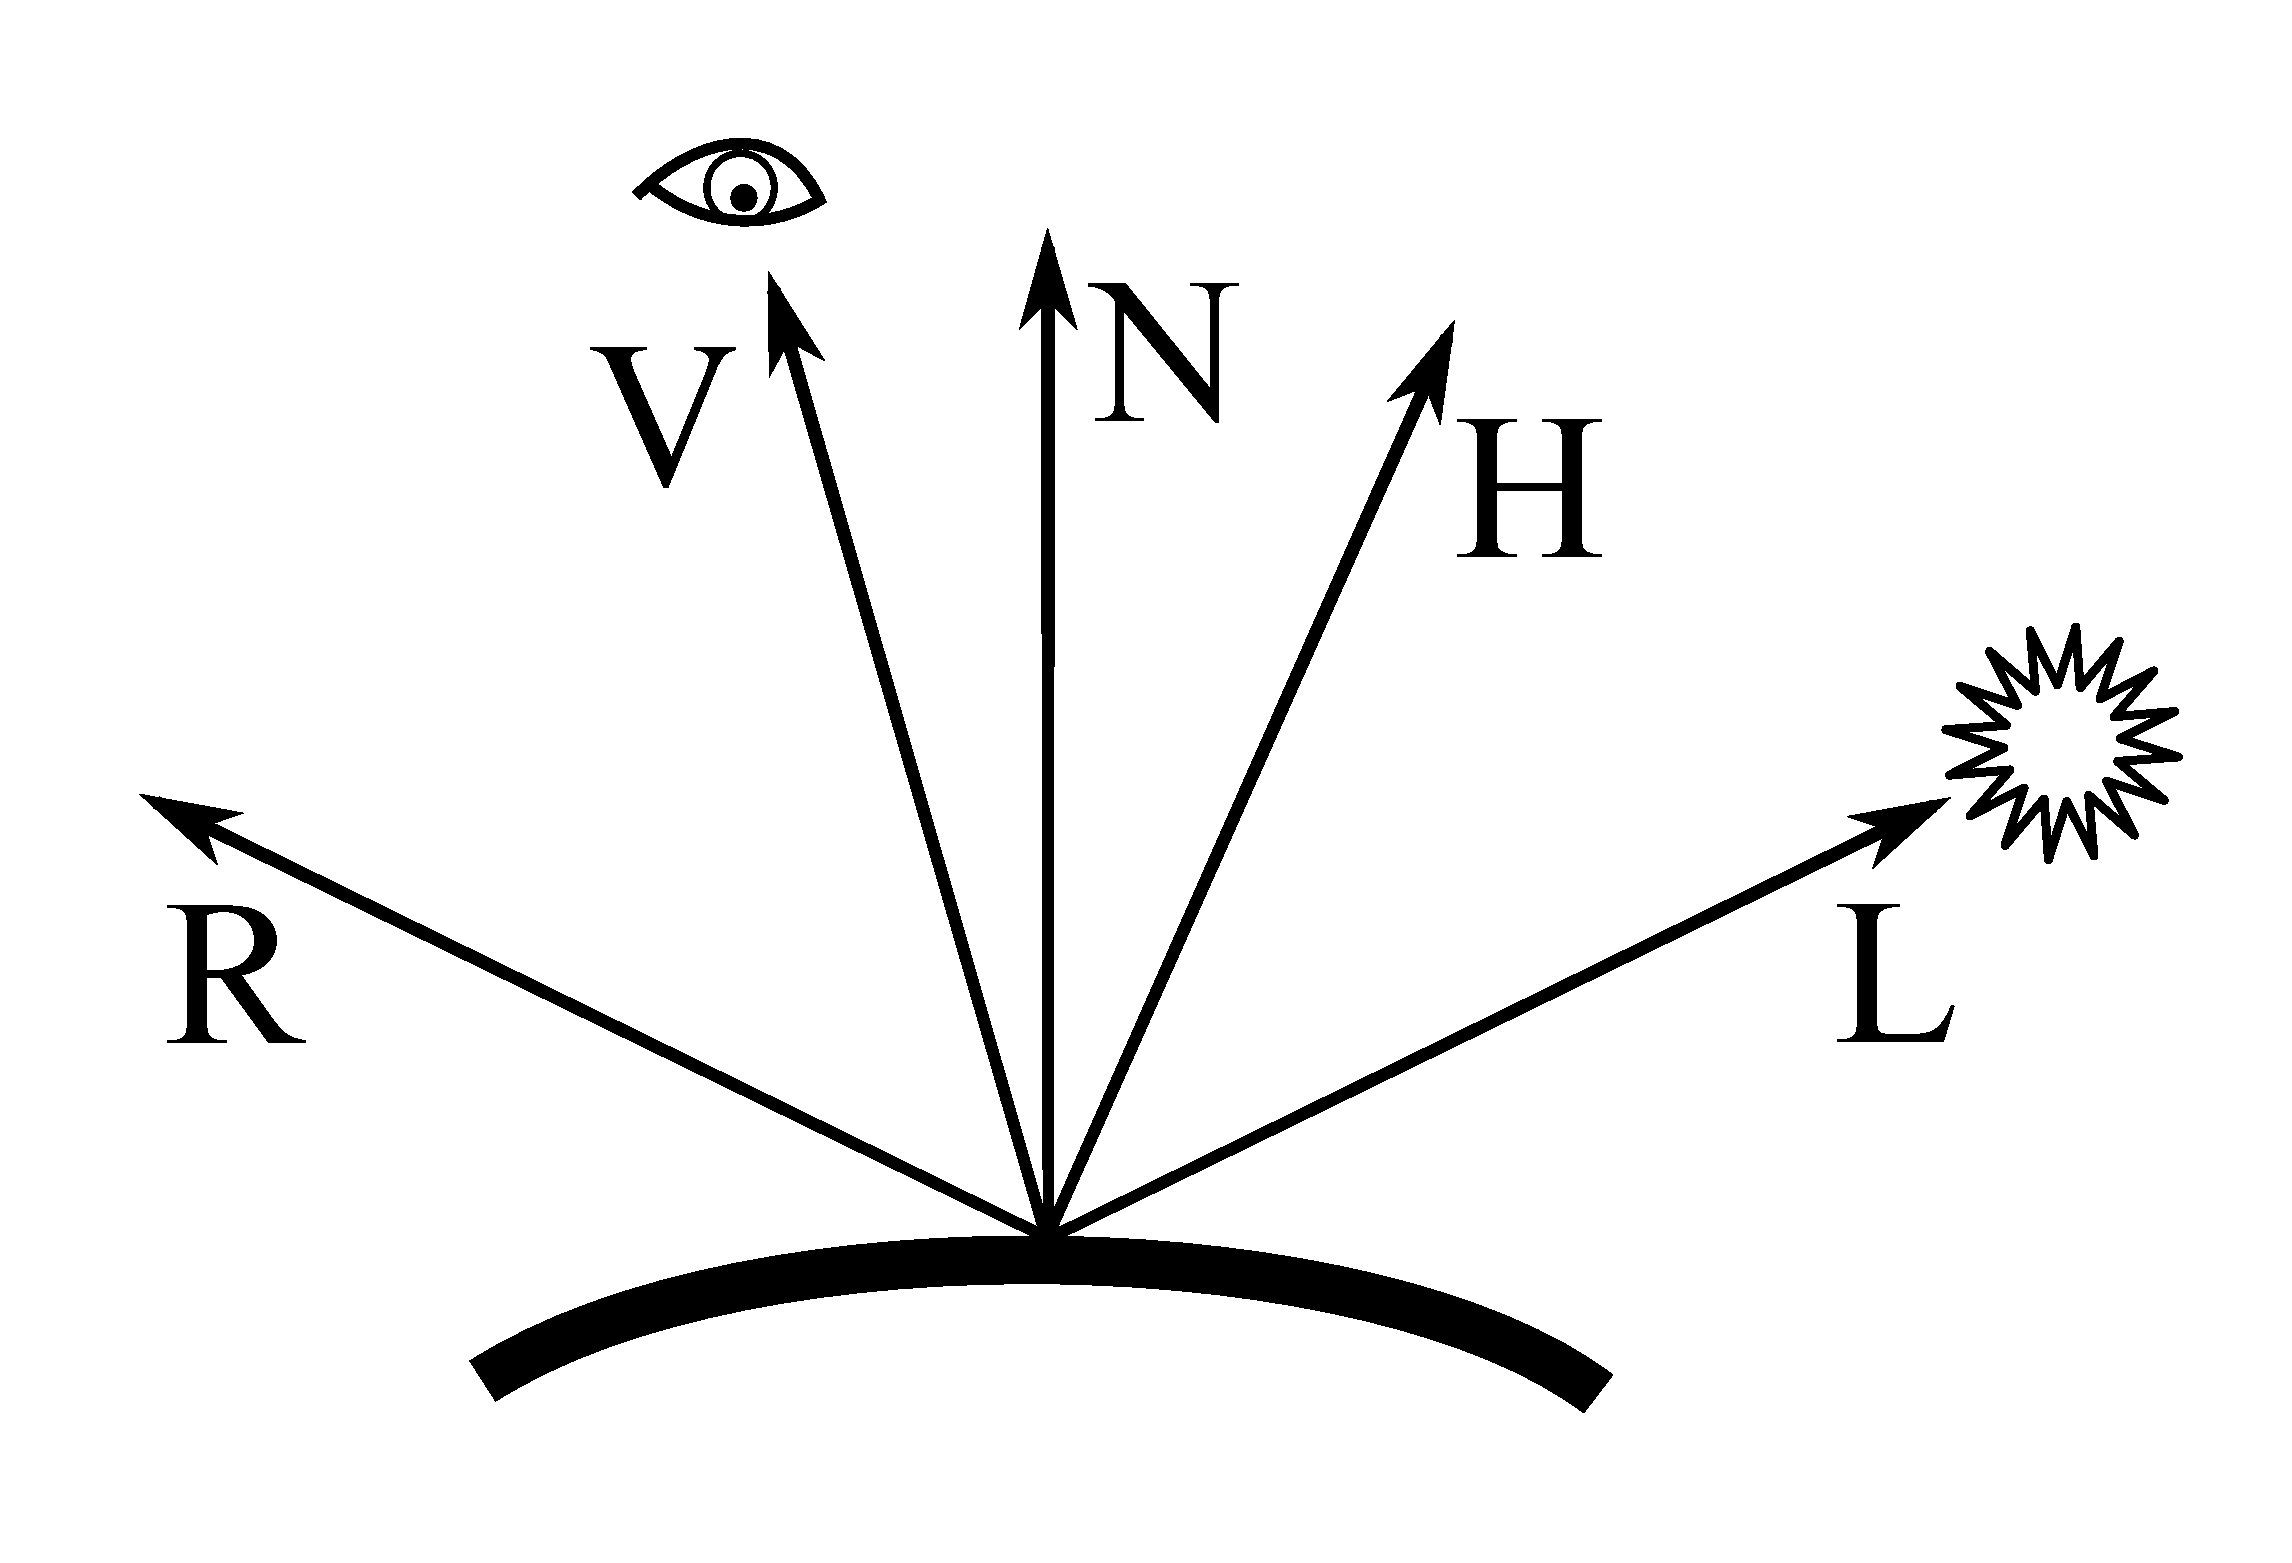
\includegraphics[width=\textwidth]{brdf}
	\caption[Bidirectional Reflectance Distribution Function]{Bidirectional Reflectance Distribution Function $f$\protect\footnotemark}
\end{figure}

\footnotetext{Quelle: http://commons.wikimedia.org/wiki/File:Blinn\_Vectors.svg}
\clearpage

\subsection{Cook-Torrance Modell}

Das Reflexionsverhalten von Oberflächen wird in der Realität wesentlich von der Oberflächenbeschaffenheit des Materials aber auch dem Material an sich bestimmt. Ein realistisches Reflexionsmodell muss diese Oberflächenbeschaffenheiten und das Material berücksichtigen. Je mehr Oberflächenparameter in das Beleuchtungsmodell einfließen können, desto realistischer und plausibler das Ergebnis.

Beispielsweise spiegeln polierte Oberflächen die Umgebung und erhalten Glanzlichter bei direkter Beleuchtung. Irreguläre rauhe Oberflächen streuen das einfallende Licht ungleichmäßig in alle Richtungen. Wachs oder Haut lässt das Licht zum Teil in das Material eindringen und zerstreut es. Die glänzenden Reflexionen von metallischen Oberflächen werden durch die Leitfähigkeit des Materials bestimmt (siehe \fref{sec:pbr-dielektisch}).

Viele Material- und Oberflächenparameter sind im Offline-Verfahren, und besonders in Echtzeitverfahren, nicht simulierbar. In Echtzeitverfahren ist es beispielsweise nicht praktikabel die mikroskopischen Unebenheiten, genannt \textit{Mikrofacetten} oder \textit{Microfecets} (siehe \fref{fig:microfacet}), exakt zu berechenen. Entsprechend wurden einige approximierende Microfacet Modelle entwickelt, die die Interaktion des Lichts mit den Facetten, realistisch abbilden können.

\begin{figure}
	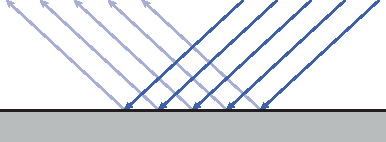
\includegraphics[width=.5\textwidth]{roughness0}
	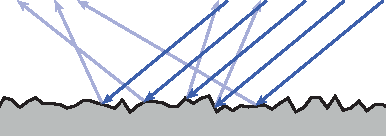
\includegraphics[width=.5\textwidth]{roughness1}
	\caption[Rauheit]{links: $m = 0$; rechts $m = 1$}\label{fig:microfacet}
\end{figure}

Eines von ihnen ist das Cook-Torrance Modell \parencite{Cook1981}, welches mit dem Ziel entwickelt wurde die physikalischen Reflexionseigenschaften von rauhen und glatten Oberflächen realistischer abzubilden, als die klassischen Modelle es ermöglichen \parencite[Seite 40]{Ngan2004}. Da sich das Cook-Torrance Modell auf spekulare Reflexionen konzentriert, verwenden wir das Cook-Torrance Modell auschließlich zur Berechnung des spekularen Anteils $f_s$ der BRDF. Der diffuse Anteil $f_d$ wird durch das klassische Lambert'sche Modell abgebildet und nicht weiter betrachtet. Denkbar sind aber auch andere Modelle für die diffuse Reflexion. In \fref{eq:cook-torrance-model} wird das Modell formal dargestellt
.
\begin{align}
	\label{eq:cook-torrance-model}
	% \caption{Cook-Torrance Illumination}
	f_s(\vV,\vL) = \frac{\mathcal{F}(\vV,\vL)D(\vV,\vL)G(\vV,\vL)}{4(\vN \cdot \vV)(\vN \cdot \vL)}
\end{align}

Der spekulare Beitrag $f_s$ wird durch die drei Faktoren bestimmt: Dem Fresnel $\mathcal{F}$ Term, der Mikrofacetten Richtungsverteilung (Microfacet Distribution Function), $D$ und der geometrischen Abschwächung (Geometrical Attenuation) $G$. Die Auswahl der konkreten Approximationen folgt der aus \cite[Seite 3]{Karis2013}.

\subsubsection[Fresnel]{Fresnel $\mathcal{F}$}
Der Fresnel Effekt beschreibt die Beobachtung, dass Oberflächen stärker reflektieren, umso flacher der Betrachtungswinkel wird. Als Approximation wurde die \textit{Schlick Approximation} \parencite{Schlick1994} gewählt. In \cite{Lagarde2012} wurde eine weitere Modifikation vorgeschlagen, um den Berechnungsaufwand im Shader zu reduzieren. Diese findet hier ebenso ihre Anwendung. $F_0$ beschreibt die Reflektanz (als Farbwert) für parallel zur Normale $\vN$ einfallendes Licht.

\begin{align}
	\label{eq:fresnel-schlick}
	\mathcal F(\vV,\vL) = F_0  + (1 - F_0) 2^{(-5.55473 (\vV \cdot \vH) - 6.98316 (\vV \cdot \vH))}
\end{align}


\subsubsection[Mikrofacetten Normalverteilung]{Mikrofacetten Normalverteilung $D$} 
Die Funktion $D$ beschreibt die statistische Normalverteilung der Ausrichtung der Mikrofacetten entsprechend der Winkelhalbierenden $\vH$. Die Mikrofacetten von glatten Oberflächen sind überwiegend gleich ausgerichtet, so dass Licht hauptsächlich entlang $R$ reflektiert wird. Raue Oberflächen besitzen eher zufällig ausgerichtete Mikrofacetten, so dass das reflektierte Licht breiter gestreut wird. Die Rauheit der Oberfläche wird mit $m$ im Intervall $[0,1]$ ausgedrückt. Zur Approximation von $D$ finden sich wiederum eine Vielzahl von Modellen. Die Implementierung verwendet das als \textit{GGX} in \cite{Walter2007} vorgestellte Modell (siehe \fref{eq:ggx}).

\begin{align}
	\label{eq:ggx}
	D(\vV,\vL) = \frac{m^4}{ \pi \left(\left( \vN \cdot \vH \right)^2\left(m^4 - 1\right) + 1\right)^2}
\end{align}


\subsubsection[Geometrische Abschwächung]{Geometrische Abschwächung $G$} 
$G$ beschreibt einen Faktor, der die Tatsache simuliert dass Mikrofacetten sich gegenseitig einfallendes oder reflektiertes Licht blockieren und sich somit gegenseitig schattieren ($G_1(\vL)$) oder Reflexionen maskieren ($G_1(\vV)$) können. Verwendet wird eine modifizierte Version der \textit{Schlick} Approximation, damit sie sich dem physikalisch präziseren Smith Modell annähert. Eine genauere Analyse des Smith Modells findet sich in \cite[Kapitel 6, Seite 33]{Heitz2014}.

\begin{align}
	\label{eq:geometric-schlick}
	k &= \frac{(m + 1)^2}{8}\\
	G_1(\vV) &= \frac{\vN \cdot \vV}{(\vN \cdot \vV)(1-k)+k}\\
	G_1(\vL) &= \frac{\vN \cdot \vL}{(\vN \cdot \vL)(1-k)+k}\\
	G(\vV,\vL) &= G_1(\vV) G_1(\vL)
\end{align}


\subsubsection{Dielektische und metallische Materialien}\label{sec:pbr-dielektisch}

\begin{figure}
	\includegraphics[width=.5\textwidth]{dielectric}
	\includegraphics[width=.5\textwidth]{metallic}
	\caption[Dielektische und metallische Materialien]{links: Plastik; rechts: Messing}
	\label{fig:dielectric-metallic}
\end{figure}

In der Natur lassen sich Substanzen bezüglich ihrer Leiteigenschaften in drei Kategorien einteilen: Nichtleiter (Dielektrikum oder Isolatoren), Halbleiter und Leiter (u.A. metallische Substanzen). Ohne auf die physikalischen Details einzugehen (Details in \cite[Abschnitt: Glanz und Farbe der Metalle]{Zawischa2011}) unterscheiden sich metallische und dielektrische Materialien in ihrem spekularem Reflexionsverhalten. Dielektrische Materialien besitzen ausschließlich weiße spekulare Reflexionen\footnote{unter weißem Licht} während metallische Materialien über ein Farbspektrum spekular reflektieren \parencite[Abschnitt: Specular]{Lagarde2011a}(siehe \fref{fig:dielectric-metallic}).

In der Implementierung wird dies über eine Justierung des $F_0$ Wertes aus dem Fresnel-Term $\mathcal{F}$ abgebildet. Für metallische Materialien wird $F_0$ auf die Grundfarbe (Albedo) des Materials gesetzt und die Grundfarbe auf schwarz, ansonsten wird $F_0$ auf weiß gesetzt (Die Idee basiert auf der \textit{Unreal Engine 4} Implementierung, Stand 2015).

\section{Praktische Umsetzung}
\label{sec:pbr-umsetzung}

Wie Eingangs erwähnt erfordert die Umstellung auf \ac{PBR} eine Anpassung in der Produktion und der Render"-pipeline. Während Diffuse- bzw. Albeo-Texturen sowie Normalentexturen bereits üblich sind, ist es für die Albedo Texturen wichtig, dass sie von jeglicher vorberechneter Beleuchtung bereinigt sind, damit die grundlegenden Texturen in allen Beleuchtungssituationen anwendbar sind (Details in \cite{Lagarde2011}). Die Implementierung der \ac{PBR} Pipeline wird im \fref{sec:src-pipeline} aufgelistet. Im Folgenden eine kurze Übersicht über die praktischen Grundlagen der Implementierung.

\subsection{Eingangsparameter}

\begin{figure}
\centering
	\includegraphics[width=\textwidth]{shots/pbr02}
	\caption{Von links nach recht ansteigender Rauheitswert}
	\label{fig:pbr-roughness}
\end{figure}

Als Eingangsparameter verwendet die Pipeline der Implementierung dieser Arbeit folgende Größen:
\begin{itemize}
\item Albedo-Textur im sRGB Farbraum (\fref{fig:pbr-albedo-tex})
\item Normalen-Textur mit Oberflächennormale im Tangenten-Raum kodiert in RGB (\fref{fig:pbr-normale-tex})
\item Roughness-Textur ($m$) in Graustufen (\fref{fig:pbr-roughness-tex})
\item Metallic-Textur in Graustufen für die Unterscheidung von dielektrischen und metallischen Oberflächen (\fref{fig:pbr-metalmask-tex})\footnote{Entspricht einer Maske, 0 = nicht metallisch, 1 = metallisch}
\end{itemize}

\begin{figure}
\centering
\begin{subfigure}{0.24\textwidth}
	\includegraphics[width=\textwidth]{Door_IronDungeonDoor_1k_alb}
	\caption{Albedo-Textur}\label{fig:pbr-albedo-tex}
\end{subfigure}
\begin{subfigure}{0.24\textwidth}
	\includegraphics[width=\textwidth]{Door_IronDungeonDoor_1k_n}
	\caption{Normalen-Textur}\label{fig:pbr-normale-tex}
\end{subfigure}
\begin{subfigure}{0.24\textwidth}
	\includegraphics[width=\textwidth]{Door_IronDungeonDoor_1k_g}
	\caption{Roughness-Textur}\label{fig:pbr-roughness-tex}
\end{subfigure}
\begin{subfigure}{0.24\textwidth}
	\includegraphics[width=\textwidth]{Door_IronDungeonDoor_1k_h}
	\caption{Metal-Mask-Textur}\label{fig:pbr-metalmask-tex}
\end{subfigure}
\caption{Beispiel eines Textur-Sets}
\label{fig:pbr-texturen}
\end{figure}


\subsection{Renderverfahren}

Als Renderverfahren wurde das als \textit{Deferred Shading} bekannte Verfahren gewählt, da es effizienter als \textit{Forward Shading} in der Lichtberechnung mit vielen Lichtern ist. Dazu wird vor der Berechnung der Schattierung der Oberflächen die Geometrie gerendert. In diesem Renderschritt werden die Oberflächenattribute wie Albedo-Farbe, Roughness und Normale in Texturen gerendert, kombiniert oft \textit{G-Buffer} genannt. Dieser \textit{G-Buffer} dient anschließend im Shading Renderschritt als Grundlage für die Berechnung. In diesem Schritt werden die Lichter mit Stellvertreter Geometrien gerendert. Für jedes so erzeugte Fragment wird die gewählte \ac{BRDF} mit Hilfe der Lichtparameter und der Parameter aus dem G-Buffer ausgewertet. In der fortlaufenden Pipeline werden die Farbwerte im HDR-Raum behandelt. Im abschließenden Tone-Mapping Schritt werden die Farbwerte vom HDR-Raum auf den linearen (s)RGB Raum übertragen. Weiterführende Details finden dazu finden sich in der Implementierung zu dieser Arbeit oder in \cite{Shishkovtsov2005}.

\subsection[Indirekte Beleuchtung]{Indirekte Beleuchtung mit \acl{IBL}}\label{sec:pbr-ibl}

Bisher wurde nur die direkte Beleuchtung von Materialien betrachtet. Aber ein weiterer wesentlicher Beitrag zum realistischen Eindruck ist die sogenannte indirekte Beleuchtung. Indirekte Beleuchtung beschreibt die physikalische Tatsache, dass Objekte nicht nur direkt von Lichtquellen beleuchtet werden, sondern selbst wieder Licht reflektieren. Entweder trifft das reflektierte Licht in das Auge des Betrachters, so dass Objekte für uns sichtbar werden, oder wiederum auf andere Objekte. Letzteres führt dazu, dass Oberflächen, durch das von anderen Oberflächen reflektierte Licht, zusätzlich beleuchtet werden \warn{Bild}. Diese wechselseitige Interreflexion wird unter dem Begriff indirekte Beleuchtung zusammengefasst.

Bisher haben wir in \fref{eq:brdf-dekonstruiert} ausschließlich die \ac{BRDF} mit direkter Beleuchtung betrachtet, aber die \ac{BRDF} lässt sich wie in \ref{eq:brdf-indirect-dekonstruiert} um Beiträge aus ambienten bzw. indirekten Beleuchtungstermen erweitern. Da spekulare Reflexionen kein Sonderfall von glatten Oberflächen sind \parencite{Hable2010}, lohnt ein generelles Verfahren zur Berechnung des indirekten Beitrags $f_{indirect}$. 

\begin{align}
	% \caption{Dekonstruierte BRDF}
	\label{eq:brdf-indirect}
	f   &= f_d + f_s\\
	\intertext{Erweiterung von $f_d$ und $f_s$ um ambienten Beitrag:}
	{f_d}^{\prime} &= f_{d_{indirect}} + f_{d_{direct}}\\
	{f_s}^{\prime} &= f_{s_{indirect}} + f_{s_{direct}}\\
	\label{eq:brdf-indirect-dekonstruiert}
	f^{\prime}   &= \underbrace{f_{d_{indirect}} + f_{s_{indirect}}}_{f_{indirect}} + \underbrace{f_{d_{direct}} + f_{s_{direct}}}_{f_{direct}}
\end{align}

Idealerweise lässt sich die Pipeline um ein umfassendes \acf{GI}\footnote{\acl{GI} Synonym für indirekte Beleuchtung.} Verfahren erweitern, das die wechselseitigen Interreflexionen aller Objekte im Raum über ein möglichst breites Frequenzenband\footnote{niedrige Frequenzen = diffuse Reflexion $f_{d_{indirect}}$; hohe Frequenzen = spekulare Reflexion $f_{s_{indirect}}$} hin abdeckt. Doch voll dynamisches \ac{GI} ist in Echtzeit immer noch nicht vollends praktikabl. Verfahren wie \ac{SVOGI} \parencite{Lin2013} erlauben zwar auch spekulare Reflexionen sind aber praktisch nur auf Highend Hardware durchführbar.

Deswegen findet ein vorberechnetes Verfahren Anwendung. Ein weiterer Grund ist, dass die Implementierung einfacher ist. Zum Einsatz kommt ein erweitertes \acf{IBL} Verfahren, dass die Umgebungstexturen im Preprozess für die unterschiedlichen Frequenzen vorintegriert. Die Vorintegration läuft aktuell noch nicht direkt in der Pipeline, sondern wird offline mit dem von Sébastien Lagarde modifiziertem Programm \textit{AMD Cubemapgen} durchgeführt \parencite{Lagarde2012a}. Dazu wird eine HDR-Cubemap in das Programm geladen und mit den passenden Einstellungen gefiltert. Das Resultat ist eine \ac{PMREM} die dann geladen und in der Auswertung der \ac{BRDF} verwendet wird.

\paragraph{Pre-Filtered Mipmapped Radiance Environment Map} Betrachten wir die Reflexion an einem Oberflächenpunkt aus Sicht des Betrachters, so bestimmt sich die Reflexion aus der Streuung des reflektierten Sichtstrahls ($\vR$). Ein perfekter Spiegel reflektiert den Sichtstrahl ohne jegliche Streuung während rauhe Oberflächen den Strahl mit zunehmender Rauheit entsprechend breiter streuen, bis hin zur ausschließlich diffusen Streuung.

Betrachten wir diffuse und spekulare Reflexionen als diffuse und spekulare indirekte Beleuchtung der Umgebung, lässt sich aus \fref{eq:brdf-indirect-dekonstruiert} folgern, dass sich Reflexionen mit dem $f_{indirect}$ Term abbilden lassen. Für die Rauheit der Oberflächen wurde $m$ als Einflussgröße für den spekularen Anteil der \ac{BRDF} eingeführt. Betrachten wir Umgebungstexturen (\textit{Environment Maps}) als Repräsentation des einfallenden Lichts, können wir Umgebungstexturen für die Berechnung des ambienten Terms $f_{indirect}$ verwenden. Entsprechend der Oberflächen Rauheit muss dafür das einfallende Licht über einen Ausschnitt der Hemisphäre aufgesammelt werden. Dies entspricht der Auswertung der \ac{BRDF} über dem entsprechenden Raumwinkel $\Omega$ (siehe \fref{eq:ambient-integral}). Dies führt zu dem in \fref{eq:ambient-integral} aufgeführtem Integral.

\begin{equation}
	\label{eq:ambient-integral}
	R = \int\limits_{\Omega} f(\vV,\vL)(\vN \cdot \vL)Env(\vL)\, \mathrm{d}\omega_{\vL}\\
\end{equation}

mit $Env(\vL)$ = \text{Wert aus Umgebungstextur entlang Richtungsvektor} $\vL$

Für einen perfekt spiegeligen Oberflächenpunkt reduziert sich der Raumwinkel $\Omega$ auf einen Strahl. Mit steigender Rauheit $m$vergrößert sich der Raumwinkel bis hin zur ganzen Hemisphäre. Wird die gesamte Hemisphäre integriert, entspricht das der diffusen indirekten Beleuchtung. 

Die Auswertung für beliebige $m$ ist zur Laufzeit zu aufwändig. Deswegen wird im Vorfeld eine entsprechende Faltung (Auswertung des Integrals inklusive der \ac{BRDF}) für abgestufte Werte von $m$ im Bereich $[0,1]$ auf die Umgebungstextur angewendet. Die gefalteten Umgebungstexturen werden in den Mipmap-Stufen der Umgebungstextur gespeichert. Dies ermöglicht die Berechnung der Werte $f_{s_{indirect}}$ und $f_{d_{indirect}}$ auf Basis der gefilterten Umgebungstextur zur Laufzeit, indem wir den Rauheitswert $m$ auf die entsprechende Mipmap Stufe abbilden und den Radiance Wert $R$ der Umgebungstextur auswerten.

\begin{figure}
\centering
\begin{subfigure}{0.18\textwidth}
	\includegraphics[width=\textwidth]{grace_m00_c00}
	\caption{Basis-Textur}\label{fig:pmrem-basis}
\end{subfigure}
~
\begin{subfigure}{0.18\textwidth}
	\includegraphics[width=\textwidth]{grace_m01_c00}
	\caption{Stufe 1}\label{fig:pmrem-1}
\end{subfigure}
\begin{subfigure}{0.18\textwidth}
	\includegraphics[width=\textwidth]{grace_m02_c00}
	\caption{Stufe 2}\label{fig:pmrem-2}
\end{subfigure}
\begin{subfigure}{0.18\textwidth}
	\includegraphics[width=\textwidth]{grace_m03_c00}
	\caption{Stufe 3}\label{fig:pmrem-3}
\end{subfigure}
\begin{subfigure}{0.18\textwidth}
	\includegraphics[width=\textwidth]{grace_m04_c00}
	\caption{Stufe 4}\label{fig:pmrem-4}
\end{subfigure}
\caption[Beispiel einer PMREM Textur]{Basis-Textur (\subref{fig:pmrem-basis}) und die ersten vier \ac{PMREM} Stufen einer Fläche der Environment Cubemap (\subref{fig:pmrem-1} - \subref{fig:pmrem-4})}
\end{figure}

\warn{Engine-Bild diffuse ambient, spekular ambient}

\section{Wo wird es eingesetzt?}
\label{sec:pbr-wo}

\ac{PBR} findet inzwischen in folgenden kommerziellen Engines Verwendung:
\begin{itemize}
\item CryEngine (Crysis 3) \parencite{Schulz2014}
\item Unreal Engine 4 \parencite{Martin2012}
\item Frostbite (Battlefield 3 \& 4) \parencite{Lagarde2014}
\item IW-Engine (Call of Duty) \parencite{Lazarov2011}
\item EVE Online Engine \parencite{CCP2014}
\item Killzone: Shadow Fall \parencite{Drobot2013}
\item FOX Engine (Metal Gear Solid) \footnote{http://www.eurogamer.net/articles/digitalfoundry-tech-analysis-mgs5-fox-engine [Abgerufen: \today]}
\end{itemize}


%%%%%%%%%%%%%%%%%%%%%%%%%%%%%% Anwendungsbeispiele
\chapter{Anwendungsbeispiele}
\label{chap:anwendung}

Es folgt eine exemplarische Implementierung eines Tone-Map Render"-schritts. Die Aufgabe des Render"-schritts besteht darin eine HDR-Textur auf einen vom Monitor darstellbaren RGB Farbraum abzubilden. Die Berechnung der Farbwerte wird im Shader |"res/glsl/sampling/tonemap.frag"| vorgenommen und ist hier, mit einem Verweis auf die Implementierung, nicht weiter aufgeführt. Die folgende Implementierung wird schrittweise erläutert und in Teilen aus didaktischen Gründen etwas gegenüber der eigentlichen Implementierung vereinfacht. Der zusammenhängende Quellcode dieses Beispiels findet sich in \fref{lst:tonemap-pass-vollstaendig}.

\paragraph{Ressourcenverwaltung} In der Implementierung wird eine eigene |Resource| Monade zur Verwaltung der Ressourcen auf Basis des |resourcet|\footnote{https://hackage.haskell.org/package/resourcet} Pakets verwendet. In dieser |Resource| Monade lassen sich Ressourcen akquirieren (zum Beispiel mit |glResource|) und über die |Applicative| und |Functor| Instanzen kombinieren. Verlässt das Programm den Kontext der |Resource| Monade, zum Beispiel beim Beenden der Renderloop, werden alle Ressourcen über die registrierte Operation freigegeben.

\paragraph{StateVars} |StateVars| kapseln zwei IO Operationen, von der eine Operation einen Wert abfragt und und die andere Operation einen Wert setzt. Oft werden StateVars in Verbindung mit externen (foreign) Biblitheken verwendet um veränderliche Zustände zu kapseln. StateVars können als normale Haskell Datenobjekte verwendet werden. Eine Ad-Hoc Implementierung findet sich in \fref{lst:statevar}.

\newpage

\begin{haskell}[label={lst:tonemap-pass-sig},caption={\texttt{ToneMapPass} Signatur},nolol]
type ToneMapInput = (HDRSensor, Texture2D PixelHDR, Maybe (Texture2D PixelHDR))
type ToneMapOutput = (Texture2D PixelRGB8)
type ToneMapPass = RenderPass ResIO ToneMapInput ToneMapOutput
\end{haskell}

Die Eingabe in |ToneMapPass| ist ein Triple aus |HDRSensor|, einer HDR Textur |Texture2D PixelHDR| und einer weiteren optionalen HDR Textur, die additiv mit der ersten im Fragment-Shader gemischt wird. |HDRSensor| ist Teil einer |HDRCamera| und beinhaltet für das Tone-Mapping benötigte Größen, wie den Weiß-Punkt oder die Belichtung (Exposure). Die Ausgabe von |ToneMapPass| ist eine übliche RGB Textur.

\begin{haskell}[label={lst:tonemap-pass-res},caption={\texttt{ToneMapPass} Resourcen Allokation},nolol]
toneMap :: Resource ToneMapPass
toneMap = do
  emptyvao <- glResource
  boundVertexArray $= emptyvao
  fbo <- glResource
  
  pipeline <- [ $(embedShaderFile "res/glsl/sampling/drawRectangle.vert")
              , $(embedShaderFile "res/glsl/sampling/tonemap.frag")]
              `compileShaderPipeline` includePaths
  Just (FragmentShader{..}) <- traverse fragmentUniforms =<< get (fragmentShader $ pipeline^.pipelineProgram)

  outTexture <- liftIO . newIORef =<< createTexture2D GL_TEXTURE_2D (Tex2D 1 1) 1

  return $ mkStaticRenderPass $ \(sensor, sceneTex, mBloomTex) -> do
\end{haskell}

In \fref{lst:tonemap-pass-res}, dem Ressourcenblock des Renderschritts, werden die Ressourcen akquiriert, die zur Ausführung der ab \fref{lst:tonemap-pass-run-resize} beschrieben Routine notwenig sind. Dazu gehören ein Vertex Array Objekt, Framebuffer Objekt und die aus dem Vertex-Shader |drawRectangle.vert| und dem Fragment-Shader |tonemap.frag| erzeugte \textit{OpenGL} Pipeline\footnote{https://www.opengl.org/wiki/GLSL\_Object\#Program\_pipeline\_objects}. Die Uniform Variablen des Frag"-ment-Sha"-ders werden von |fragmentUniforms| als |StateVar|s gekapselt (siehe Verwendung \fref{lst:tonemap-pass-run-pipeline}). Zusätzlich wird eine ausschließlich intern verwendete |IORef| für die Ausgabetextur erzeugt. Da die verwendeten \textit{OpenGL} Texturen\footnote{erzeugt mit \texttt{glTexStorage*}} in ihrer Größe unveränderlich sind, muss für neue Ausgabegrößen eine neue Textur erzeugt werden (siehe \fref{lst:tonemap-pass-run-resize}). |resizeTexture2D| nimmt diese Operation vor, in dem es die benötigten Werte der alten Textur übernimmt und eine neue Textur neuer Größe erzeugt. Die alte Textur wird freigegeben. Dieses Texturobjekt speichern wir uns für den nächsten Aufruf in der |IORef|.

\begin{haskell}[label={lst:tonemap-pass-run-resize},caption={[ToneMapPass Größenanpassung des Framebuffers]\texttt{ToneMapPass} Größenanpassung des Framebuffers},nolol]
    target <- get outTexture
    when (target^.textureDimension /= sceneTex^.textureDimension) $ do
      let V2 w h = sceneTex^.asRectangle.extend
      newtarget <- (\t -> resizeTexture2D t w h) =<< get outTexture
      outTexture $= newtarget
      void $ attachFramebuffer fbo [mkAttachment newtarget] Nothing Nothing
    boundFramebuffer RWFramebuffer $= fbo
\end{haskell}

Die Größenanpassung der Ausgabetextur erzeugt eine neue Textur, so dass die neue Textur noch dem Framebuffer neu angefügt werden muss (\fref{lst:tonemap-pass-run-resize}).

\begin{haskell}[label={lst:tonemap-pass-run-pipeline},caption={\texttt{ToneMapPass} Zuweisung an Uniform Variablen},nolol]
    boundProgramPipeline $= pipeline^.pipelineProgram

    iScene $= sceneTex
    iBloom $= mBloomTex
    iHdrSensor $= sensor
\end{haskell}

In \fref{lst:tonemap-pass-run-pipeline} wird die erzeugte Shaderpipline für diesen Renderschritt global aktiviert und den, in |StateVar|s gekapselten, Uniform Variablen des Fragment-Shaders Werte des Sensors zugewiesen. Zusätzlich werden die Texturen an die jeweiligen Texture-Einheiten von \textit{OpenGL} gebunden. Die Zuweisung ist auch entsprechend in den |StarVar|s gekapselt.

\begin{haskell}[label={lst:tonemap-pass-run-draw-and-out},caption={\texttt{ToneMapPass} Draw-Call und Textur ausgeben},nolol]
    glDrawArrays GL_TRIANGLES 0 3

    get outTexture
\end{haskell}

Abschließend wird der Draw-Call abgesetzt und die nun von \textit{OpenGL} gefüllte Textur als Ausgabe zurück gegeben (\fref{lst:tonemap-pass-run-draw-and-out}).


%%%%%%%%%%%%%%%%%%%%%%%%%%%%%% Analyse
\chapter{Resultat}
\label{chap:resultat}

In der vorliegenden Arbeit wurde eingangs in \fref{chap:engine-uebersicht} aus den gestiegenen Anforderungen an die Softwareprojekte in der Spielebranche die Motivation entwickelt, neue Mittel und Wege für das Beherrschen der zunehmenden Komplexität zu suchen. Die zunehmende Komplexität in Softwareprojekten erhöht die Wahrscheinlichkeit des Scheiterns von diesen Projekten. Es wurde festgestellt, dass die Programmiersprache das wichtigste Kommunikationsmittel unter den Softwareentwicklern ist. Dementsprechend spielt die Programmiersprache eine zentrale Rolle in Softwareprojekten, sie bestimmt die Kommunikation aber auch die Softwarearchitektur und die Möglichkeiten der Entwickler.

Jede Branche und jedes Projekt besitzt eigene individuelle Anforderungen und Herausforderungen. In der Grafik-Engine-Entwicklung stellen die Grafik-\ac{API}s die Kernherausforderungen. In \fref{chap:modern-opengl} wurde am Beispiel von \textit{OpenGL} die Entwicklung der Grafik-\ac{API} betrachtet und welche Herausforderungen und Möglichkeiten diese Schnittstelle mit sich bringt.

\fref{chap:loesungen-durch-fp} zitierte Entwicklergrößen aus der Spielebranche. Die getroffenen Aussagen geben die aktuellen Probleme in der Spiele- und Engine-Entwicklung wieder. Es wurde gezeigt, dass viele wesentlichen Probleme, die sich in den Industriesprachen C++ / C# oder Java auftun, in anderen Sprachen entweder konzeptionell keine Probleme darstellen oder bereits gelöst sind. Diese Diskussion wird in diesem Kapitel in \fref{xp:haskell} noch einmal abschließend aufgegriffen und um persönliche Einschätzungen des Autors erweitert.

% Aus der Motiviation heraus neue Wege und Konzepte für aktuelle Probleme in der Engine-Entwicklung zu su

\section{Diskussion der Implementierung}

\section{Erfahrungen mit Haskell}\label{sec:xp-haskell}

\subsection{Vorteile von Haskell}

{\Huge Just Notes}\\
Argument performance. auch wenn engines und echtzeit performance kritisch sind, gibt es hotspots.
Der Gründer von Epic Games (Unreal Engine) würde 10\% der Performance für 10\% mehr Produktivität opfern \parencite[Seite 20]{Sweeney2006} % Next Mainstream Programming Language

Bezüglich der Implementierung eines Renderschritts wurde auf eine Abstraktion der Grafik-API verzichtet, so dass Implementierungen direkt in OpenGL umgesetzt sind.

opt-in extensions

führt aber zu eher imperativen (opengl) implementierungen der einzelnen renderschritte. Meinung

\subsection{Probleme bei Haskell}\label{sec:probleme-haskell}

Die produktive Verwendung von Haskell bringt aber auch einige Probleme mit sich. Oft sind die Probleme aber eher organisatorischer und menschlicher Natur. Zum einen sind die funktionalen Konzepte im Vergleich zu den beispielsweise OOP Konzepten nicht auf breiter Front bekannt und erfordern auch oft neue Denkmuster. Da die bestehenden Denkmuster sich jahrelang verfestigen konnten, dürften neue Denkansätze auf einigen Widerstand stoßen. Das schrittweise Einführen von Haskell dürfte auch in Unternehmensumgebungen naturgemäß einige Widerstände und Skepsis mit sich bringen.

Generell ist das schrittweise Einführen (Drop In Replacement) von Haskell aber auch praktisch nicht immer einfach. Während in modernen Serverarchitekturen sich selektiv einige kleine isolierte Dienste mit Haskellimplementierungen ersetzen ließen, dürfte sich dies bei monolithischen Projekten als schwerer herausstellen. Auch die Verknüpfung von Haskell mit C++, in der Spieleindustrie Quasi-Standard, ist noch nicht umfassend gelöst.

Tools (voll integrierte entwicklungsumgeben - abseits von Emacs)


Es lässt sich durchaus schlussfolgern, dass Haskell die richtigen Lösungen (z.B.: Unveränderlichkeit von Daten, |Maybe| statt \texttt{NULL}, \textit{rein funktional} als Grundprinzip) für viele Probleme in komplexen Softwareprojekten bereits mit sich bringt. Und deswegen stellen Bindings zu komplexen externen Frameworks keine optimale Lösung dar, auch wenn dies oft aus kurz bis mittelfristigen Gründer der Produktivität immer noch erforderlich ist. Dies stellt ein gewisses Henne-Ei-Problem dar: Auf Grund der 

Abstraktion ermöglicht optimierungen des Compilers:
Mehr anwendung von haskell, mehr workforce für den compiler, bessere optimierungen
low hangig fruits in c vermutlich schon abgefisch, in ghc noch viele bereiche offen


%%%%%%%%%%%%%%%%%%%%%%%%%%%%%% Ausblick
\include{chapter/10-ausblick}

%%%%%%%%%%%%%%%%%%%%%%%%%%%%%% Appendix

\appendix

%%%%%%%%%%%%%%%%%%%%%%%%%%%%%% Bib

%%%%%%%%%%%%%%%%%%%%%%%%%%%%%% Bib
\nocite{*}
%\bibliographystyle{natdin}
%\bibliographystyle{geralpha}
%\bibliographystyle{apalike}
\bibliographystyle{jurabib}
%%\addtocontents{toc}{\protect\vspace{\beforebibskip}}
\clearpage\addcontentsline{toc}{chapter}{\refname}
\bibliography{bib/references} 



%%%%%%%%%%%%%%%%%%%%%%%%%%%%%% Quellen
\chapter{Quellen}

\section[ToneMapPass]{\texttt{ToneMapPass}}
\label{sec:src-tonemappass}

\begin{haskell}[label={lst:tonemap-pass-vollstaendig},caption={[ToneMapPass vollständig]\texttt{ToneMapPass} vollständig}]
type ToneMapInput = (HDRSensor, Texture2D PixelHDR, Maybe (Texture2D PixelHDR))
type ToneMapOutput = (Texture2D PixelRGB8)
type ToneMapPass = RenderPass ResIO ToneMapInput ToneMapOutput

toneMap :: Resource ToneMapPass
toneMap = do
  emptyvao <- glResource
  boundVertexArray $= emptyvao

  pipeline <- [ $(embedShaderFile "res/glsl/sampling/drawRectangle.vert")
              , $(embedShaderFile "res/glsl/sampling/tonemap.frag")]
              `compileShaderPipeline` includePaths

  Just (FragmentShader{..}) <- traverse fragmentUniforms =<< get (fragmentShader $ pipeline^.pipelineProgram)

  outTexture <- liftIO . newIORef =<< createTexture2D GL_TEXTURE_2D (Tex2D 1 1) 1
  fbo <- glResource
  return $ mkStaticRenderPass $ \(sensor, sceneTex, mBloomTex) -> do
    target <- get outTexture
    when (target^.textureDimension /= sceneTex^.textureDimension) $ do
      let V2 w h = sceneTex^.asRectangle.extend
      newtarget <- (\t -> resizeTexture2D t w h) =<< get outTexture
      outTexture $= newtarget
      void $ attachFramebuffer fbo [mkAttachment newtarget] Nothing Nothing

    boundFramebuffer RWFramebuffer $= fbo

    glDisable GL_DEPTH_TEST
    glDepthMask GL_FALSE
    glDepthFunc GL_ALWAYS
    glDisable GL_BLEND
    glDisable GL_CULL_FACE
    glFrontFace GL_CCW

    boundVertexArray $= emptyvao
    boundProgramPipeline $= pipeline^.pipelineProgram

    iScene $= sceneTex
    iBloom $= mBloomTex
    iHdrSensor $= sensor
    
    glDrawArrays GL_TRIANGLES 0 3

    get outTexture
\end{haskell}

\section[StateVar]{\texttt{StateVar}}
\label{sec:src-statevar}

\begin{haskell}[label={lst:statevar},caption={[Definition StateVar]Definition \texttt{StateVar}}]
data StateVar a = StateVar (IO a) (a -> IO ())

($=) :: StateVar a -> a -> IO ()
(StateVar _ setter) $= a = setter a

get :: StateVar a -> IO a
get (StateVar getter _) = getter
\end{haskell}

\begin{landscape}
\section{Deferred PBR Pipeline Übersicht}
\label{sec:src-pipeline}
\lstinputlisting[language=Haskell,caption={Deferred PBR Pipeline Übersicht}]{src/deferred-pbr-pipeline.hs}
\end{landscape}

\chapter[DVD mit Projektquellen]{DVD mit Projektquellen}\label{chap:dvd}

Quellen auf Github mit Entwicklungsumgebung, Windows Binaries und konsolidierten Quellen:
https://github.com/MaxDaten/yage-meta/releases/tag/0.6.1


\include{chapter/99-eidesstatt}
\thispagestyle{empty}
% \cleardoublepage
\null\newpage



\end{document}
